\chapter{Matrix Algorithms}
\minitoc
Here are some of the explanation of the algorithms used in the package, at the minimal level. For details, check the references.

\section{LU Decomposition}
LU decomposition

\section{Cholesky Decomposition}
Cholesky Decomposition

\section{Geometric Transformations}
Here are the geometric transformations
rotation has determinant 1 and norm 1.

reflection has determinant -1 and norm 1.

projection has determinant != 1 or -1, the norm is not 1.

\subsection{Projection}
We are going to derive the matrix representation of the projection of a vector on another vector. 
\begin{figure*}[htp]
\centerline{
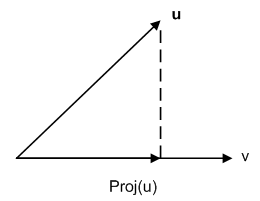
\includegraphics[bb=20 0 230 150,width=0.5\textwidth] {chap4/projection1.png}
}
\caption{Projections of u on v}
\label{figure:projection1}
\end{figure*}
Given two vectors u and v, the projection of u on v is
\[proj(u) = |u|\cos\theta \cdotp {\frac{v}{|v|}}\]
Recall that the inner product of u and v is
\[vu = v^Tu = |v||u|\cos\theta\]
by eliminating $\cos\theta$, the projection can be expressed as
\[proj(u) = |u| {\frac{v^Tu}{|v||u|}} {\frac{v} {|v|}} =
{\frac{v^Tu}{|v|}^2} v = {\frac{v^Tu}{v^Tv}} v\]
The first factor is really a scaler, so we could rewrite it
\[proj(u) = v {\frac{v^Tu}{v^Tv}} = {\frac{vv^T}{v^Tv}}u\]
So the project matrix on v is
\begin{equation}
P_v = {\frac{vv^T}{v^Tv}}
\end{equation}

where the denominator is just a scaler. Several properties of P
\begin{itemize}
\item P is symmetric, \(P^T = P\).
\item P is idempotent, \(P^2 = P\).
\end{itemize}
In numerical practice, when we deal with multiplications we don't need to store the entire P, instead we can store only the vector v. For an arbitrary vector x, 
\[Px = {{vv^T} \over {v^Tv}}x = v{{v^Tx} \over {v^Tv}} = 
{{v^Tx} \over {v^Tv}}v\]
The left factor of the above is purely a number. Similarly
\[x^TP = x^T {{vv^T} \over {v^Tv}} = {{x^Tv} \over {v^Tv}} v^T\]
Again, the left factor is a scaler. If A is a matrix, then
\[PA = {{vv^T} \over {v^Tv}}A = {{v(v^TA)} \over {v^Tv}}\]
and
\[AP = A{{vv^T} \over {v^Tv}} = {{(Av)v^T} \over {v^Tv}}\]
These formulae simplify the calculations when transforming other matrices.

Interestingly, we can extend the above result to higher dimensions. For a vector u, we want to project it to a subspace.
\begin{figure*}[htp]
\centerline{
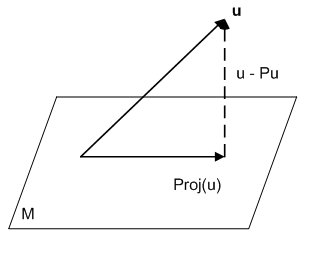
\includegraphics[bb=20 0 200 185,width=0.5\textwidth] {chap4/projection2.png}
}
\caption{Projections of u on M}
\label{figure:projection2}
\end{figure*}

\begin{lem}
Suppose \[ M = span \bigl\{v_1,\ v_2,\ \cdots,\ v_m \bigr\} \subset R^n\] where $m \leq n$ be a subspace spanned by linear independent \{$v_j$\}. The the projection matrix associated with M is
\[P = A\bigl(A^TA\bigr)^{-1}A^T\]
where $A = \bigl(v_1,\ v_2,\ \cdots,\ v_m\bigr)$, a n \texttimes m matrix, P is thus a n \texttimes n matrix. The matrix $\bigl(A^TA\bigr)^{-1}A^T$ is the pseudo inverse of A, denoted by $A^+$.
\end{lem}
\begin{proof}: For any vector u, 
\[Pu = A\bigl(A^TA\bigr)^{-1}A^Tu = A\Bigl[\bigl(A^TA\bigr)^{-1}A^Tu\Bigr] \triangleq Aw\]
So
\[Pu = (v_1,\ v_2,\ \cdots,\ v_m)
\left( \begin{array}{c} w_1\\ w_2\\ \vdots\\ w_m\\ \end{array} \right)
= \sum_{i=1}^m w_iv_i \in M \]
Next we need to prove that $u-Pu$ is perpendicular to $M$. In fact
\[A^T(u-Pu) = A^Tu - A^TPu = A^Tu - A^TA\bigl(A^TA\bigr)^{-1}A^Tu = A^Tu - A^Tu = 0\]
So $u-Pu$ is perpendicular to all ${v_j}$ and thus to $M$ too. 
It is easy to verify that $Pu$ and $u - Pu$ are perpendicular too
\[(Pu)^T(u-Pu) = u^TP^T(u-Pu) = u^TP^Tu - u^TP^TPu = 0\]
because $P^T = P$ and $P^2 = P$.
\end{proof}
Another interesting fact is the following.
\begin{figure*}[htp]
\centerline{
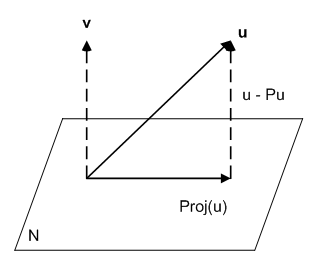
\includegraphics[bb=20 0 200 200,width=0.5\textwidth] {chap4/projection3.png}
}
\caption{Projections of u on N}
\label{figure:projection3}
\end{figure*}

\begin{lem}
Suppose $v_1,\ v_2,\ \cdots,\ v_m \in R^n$ be linear independent and $m \leq n$, let \[A = \bigl(v_1^T,\ v_2^T,\ \cdots,\ v_m^T\bigr)\] be a m \texttimes n matrix. Now consider the following subspace: \[N = \bigl\{\ x\ |\ Ax=0\ \bigr\}\] the perpendicular subspace to all $\bigl\{v_j\bigr\}$, i.e., \(N = span\bigl\{\ v_j\ |\ j=1,\ 2,\ \cdots\ m\bigr\}^\bot\). The projection matrix on N is given by
\[P = I - A^T\bigl(AA^T\bigr)^{-1}A\]
where I is the m \texttimes m identity matrix.
\end{lem}
\begin{proof}: For any vector u, 
\[A(Pu) = A\bigl(I - A^T\bigl(AA^T\bigr)^{-1}A\bigr)u = Au - AA^T\bigl(AA^T\bigr)^{-1}Au 
= Au - Au = 0\]
It implies that Pu lies in N. Furthermore, 
\[ u-Pu = A^T\left(AA^T\right)^{-1}Au \triangleq A^Tw = \bigl(v_1,\ v_2,\ \cdots\ v_m\bigr)
\left( \begin{array}{c} w_1\\ w_2\\ \vdots\\ w_m\\ \end{array} \right)
=\sum_{i=1}^m w_iv_i\]
It implies that u-Pu lies in $span\bigl\{v_i\bigr\}$ and perpendicular to N.
\end{proof}

\subsection{Reflection}
Given a vector $v$, let $M = span\bigl\{v\bigr\}^\bot$, the perpendicular space to $v$. For any vector $u$, the reflection of $u$ through M is given by
\[refl(u) = u - 2\ proj(u) = u - 2 {{vv^T} \over {v^Tv}}u =
(I - 2{{vv^T} \over {v^Tv}})u\]
\begin{figure*}[htp]
\centerline{
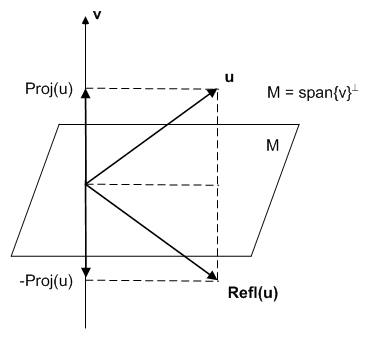
\includegraphics[bb=20 0 200 250,width=0.5\textwidth] {chap4/reflection.png}
}
\caption{Reflection of u through M}
\label{figure:reflection}
\end{figure*}
Here we use the result from last section. So the reflection matrix for M is 
\begin{equation}
Q_v = I - 2{{vv^T} \over {v^Tv}}
\end{equation}
It is easy to verify these properties:
\begin{itemize}
\item Q is symmetric, i.e., $Q^T = Q$.
\item Q is orthogonal, i.e., $Q^TQ = I$.
\item Q is involuntary, i.e., $Q^2 = I$, reflecting a vector twice should get back to the original vector.
\end{itemize}
Similar to the projection case, in numerical practice, we need to store only the vector v when applying the reflection to a vector or a matrix.

The following are several useful facts, the first one is used in the QR decomposition, the second one is used in the SVD, and the third one is used when we accumulate Householder matrices.

\begin{lem}
Given two vectors x and y with same norm, the reflection matrix that maps x to y is $Q_{x-y}$.
\end{lem}
\begin{proof}: From the above picture, if we treat u as x and refl(u) as y, it's easy to see x-y = 2proj(u) is parallel to v.
\end{proof}
If x and y don't have same norm, we could normalize both vectors first.

A typical usage of this lemma is to map a given vector to a vector of our choice, such as $e_1$, the basis in $R^n$, so that we can eliminate all components along other basis. Repeating this step we can transform a matrix to a triangular matrix.

\begin{lem}
Let x be a vector in $R^n$. For any k with $1 \leq k \leq n-2$, we can find a vector $u_k$ such that
\[Q_{u_k}x = Q_{u_k}
\left( \begin{array}{c} x_1\\ x_2\\ \vdots\\ x_k\\ \vdots\\ x_n\\ \end{array} \right) = 
\left( \begin{array}{c} x_1\\ x_2\\ \vdots\\ x_k\\ -S\\ 0\\ \vdots\\ 0\\ \end{array} \right)
\triangleq = y
\]
This means we can eliminate all components but the first two in x.
\end{lem}
\begin{proof}
If we pick 
\[S^2 = x_{k+1}^2 + x_{k+2}^2 + \cdots + x_{n}^2\]
Then x and y have the same norm. By the first lemma, 
\[u_k = x - y =
\left( \begin{array}{c} x_1\\ x_2\\ \vdots\\ x_k\\ x_{k+1}\\ x_{k+2}\\ \vdots\\ x_n\\ \end{array} \right) -
\left( \begin{array}{c} x_1\\ x_2\\ \vdots\\ x_k\\ -S\\ 0\\ \vdots\\ 0\\ \end{array} \right) =
\left( \begin{array}{c} 0\\ 0\\ \vdots\\ 0\\  x_{k+1}+S\\ x_{k+2}\\ \vdots\\ x_n\\ \end{array} \right)
\]
To avoid rounding error, the sign of S is chosen to be the same as $x_{k+1}$. Furthermore, it is easy to verify
\[ {\bigl|u_k\bigr|}_2^2 = (x_{k+1} + S)^2 + x_{k+2}^2 + \cdots + x_{n}^2
=2x_{k+1}S + 2S^2\]
\end{proof}

Lemma 3.

\subsection{Rotation}
Givens rotation matrix is defined as
\[G(i, j, c, s) = \ \ \ \bordermatrix{
    & & & & i & & & & j\cr
    & 1 \cr
    & & . \cr
    & & & 1 \cr
  i & & & & c & . & . & . & s \cr
    & & & & . & 1 \cr
    & & & & . & & . \cr
    & & & & . & & & 1 \cr
  j & & & & -s & . & . & . & c \cr
    & & & & & & & & & 1 \cr
    & & & & & & & & & & .\cr
    & & & & & & & & & & & 1\cr
}
\]
where $c^2 + s^2 = 1$. Every rotation can be decomposed into a product of a series of the above rotations.

The Householder matrix is a reflection because \(det(Q_v) = -1\). Then \(-Q_v\) is a rotation(with the angle \(\pi\)).

The Jacobi rotation is a similar transformation using G, i.e., \(G^TAG\). See the link.
\section{QR decomposition}
Let A be a n \texttimes m matrix with n > m and \(rank(A) = m\), the QR decomposition of A is \[ A = Q R \] where Q is a m \texttimes n orthogonal matrix, i.e., \(Q^TQ = I_n\), the n \texttimes n identity matrix and R is an n \texttimes n upper triangular matrix. Denote A as \[A = \bigl(\vec{a_1},\ \vec{a_2},\ \cdots,\ \vec{a_m}\bigr)\] where all \(\vec{a_j}\) are linear independent in \(R^n\) with basis $\bigl\{\vec{e_1},\ \vec{e_2},\ \cdots,\ \vec{e_n}\bigr\}$ and 
\[ \vec{a_j} = \left( \begin{array}{c} a_{1j}\\ a_{2j}\\ \vdots\\ a_{nj}\\ \end{array} \right) \] The QR algorithm, using Householder transformations, is based on the Lemma 1. After the execution, R is stored in the strictly upper triangular portion of A and R's diagonal cells are stored in a separate array. Q is stored in the lower triangular portion indirectly, actually, the vectors generating the Householder transformations are stored. In order to get Q we need to multiply these Householder transformations together. For all j, we work on the sub-matrix from j to m:
\begin{enumerate}
\item compute \(|\vec{a_j}|\), the 2-norm, square root of the sum of all components, \[\sqrt{\sum_{i=1}^{n}{a_{ij}}}\] We further select the norm to have the same sign as \(a_{jj}\) to avoid the rounding error with subtractions in the step 3.
\item overwrite \(|\vec{a_j}|\) with \(\vec{a_j} \over |\vec{a_j}|\) such that now \(\vec{a_j}\) is a unit vector. Note that we are working on the sub vector below the diagonal.
\item construct the Householder transformation for the jth sub-column so that it is mapped to \(\vec{e_j}\), the jth axis in \(R_n\). By Lemma 1, the transformation is 
\[Q_v = I - 2 {{\vec{v} \vec{v}^T} \over {\vec{v}^T \vec{v}}}\] 
where \(\vec{v} = \vec{a_j} + \vec{e_j}\). Note that \(vec{v}\) is the same as \(vec{a_j}\) except the first component is \(a_{jj} + 1\). So we just overwrite the first component of \(\vec{a_j}\) with \(a_{jj} + 1\) and thus now the jth column is \(\vec{v}\). This value will be used in the next step. As we progress j from 1 to m, the vector v has the form \(\left(0,\ 0,\ \cdots,\ v_j,\ v_{j+1},\  \cdots,\ v_n\right)\), i.e., anything above the diagonal is zero. 
\item Note that \(\vec{a_j}\) now is a unit vector, in the \(Q_v\) expression above, 
\[\vec{v}^T \vec{v} = \bigl(\vec{a_j} + \vec{e_j}\bigr)^T\bigl(\vec{a_j} + \vec{e_j}\bigr) = 
1 + a_{jj} + a_{jj} + 1 = 2\bigl(a_{jj} + 1\bigr) = 2v_j\]
So now \(Q_v\) can be expressed 
\[Q_v = I - 2 {{\vec{v} \vec{v}^T} \over {\vec{v}^T \vec{v}}} =
I - 2  {{\vec{v} \vec{v}^T} \over {2v_j}} = 
I - {{\vec{v} \vec{v}^T} \over {v_j}}\] 
where \(v_j\) is the overwritten value stored from the step 3.
\item We leave the jth column with the vector \(\vec{v}\), and apply the Householder transformation \(Q_v\) to the rest of the columns using the formula:
\[Qx = \Bigl(I - {{\vec{v} \vec{v}^T} \over v_j}\Bigr)x = 
x - {{\vec{v}^Tx} \over v_j}\vec{v}\] 
which is just a difference of two vectors x and v with a scaler.
\item store the norm from step 1 in a separate vector, this is part of the upper triangular matrix R because \(Q\vec{a_j} = |\vec{a_j}|e_j\)
\end{enumerate}
Since we store all the vectors v's in the lower portion of A, we need to multiply them to get Q.

\section{Singular Value Decomposition}
The common practice of SVD is to decompose the given matrix to a bidiagonal matrix, then compute the singular values of the reduced bidiagonal matrix.

\section{Eigen Decomposition}
scaling
\section{Reference}

For mathematical treatment, 
\begin{itemize}
\item Matrix Analysis, Horn and Johnson
\item Topics in Matrix Analysis, Horn and Johnson
\item 
\end{itemize}

For numerical algorithms
\begin{itemize}

\item Lapack documents: http://www.netlib.org/lapack/lawns/downloads/
\item Matrix Perturbation Theory, Stewart and Sun
\item Matrix Algorithms, G.W. Stewart
\item Fundamentals of Matrix Computations, D. Watkins
\end{itemize}

\begin{thebibliography}{99}

% >>>>>>>>> Book examples <<<<<<<<<
\bibitem{Demmel@1997} Demmel, J.W., {\itshape Applied Numerical Linear Algebra},
 SIAM, 1997.
\bibitem{GolubLoan} Golub, G.H., Loan, C.F., {\itshape Matrix Computations},
 3rd Edition, The Johns Hopkins University Press, 1996.
\bibitem{NumericalRecipes} Teukolsky, A., Vetterling, W.T., Flannery, B.P., {\itshape Numerical Recipes}, 3rd Edition, Cambridge University Press, 1997
\bibitem{NumericalAlgoriths} Higham, N.J., {\itshape Accuracy and Stability of Numerical Algorithms}, SIAM, 1996
\bibitem{Sparse} Sparse matrix
\bibitem{Lawn95} Lawn 95.


\end{thebibliography}
